\subsection{Notifications}

\begin{figure*}[h]
\begin{multicols}{2}
    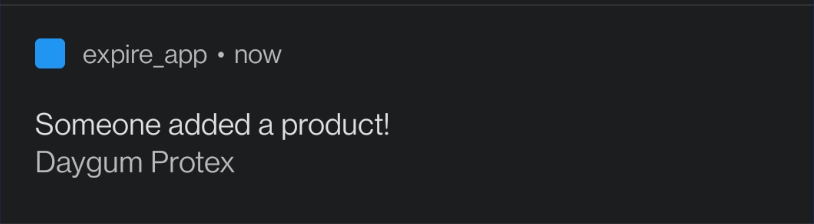
\includegraphics[width=\linewidth]{Images/notifications/new_product.png}\caption{New product added}\par 
    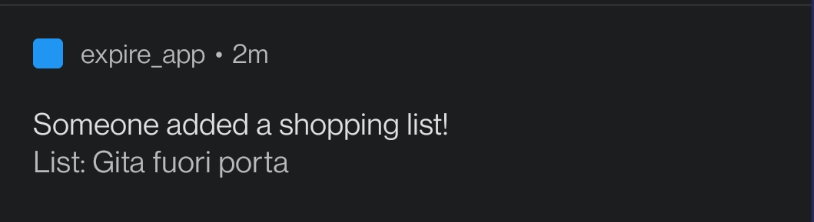
\includegraphics[width=\linewidth]{Images/notifications/new_shopping_list.png}\caption{New shopping list added}\par 
    \end{multicols}
\begin{multicols}{2}
    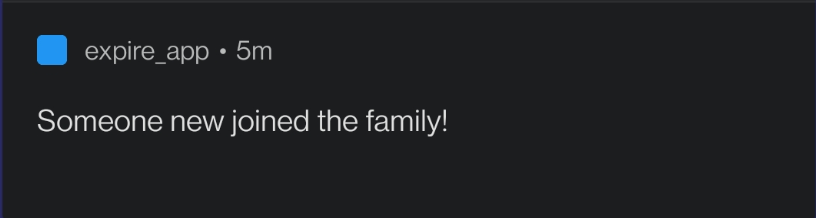
\includegraphics[width=\linewidth]{Images/notifications/new_user_family.png}\caption{New family join}\par
    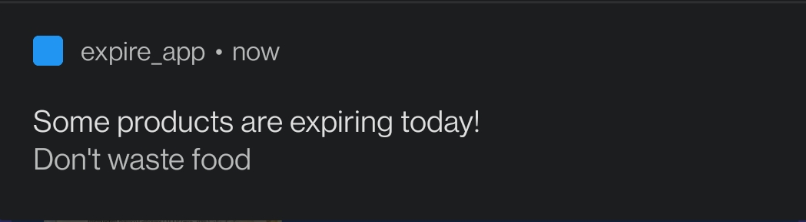
\includegraphics[width=\linewidth]{Images/notifications/expiring_notification.png}\caption{Expiration reminder}\par
\end{multicols}
\end{figure*}

Each notification is attached to its corespondent listener (Firebase trigger function) \textit{onCreate}.
\newline
\newline
\noindent\textbf{New product}
\begin{lstlisting}[caption=My Javascript Example]
exports.newProductEvent = functions.firestore
    .document("families/{familyId}/products/{productId}")
    .onCreate((snap, context) => { ... }
\end{lstlisting}
\newline
\noindent\textbf{New shopping list}
\begin{lstlisting}[caption=My Javascript Example]
exports.newShoppingListEvent = functions.firestore
    .document("families/{familyId}/shopping_lists/{shoppingListId}")
    .onCreate((snap, context) => { ... }
\end{lstlisting}
\newline
\noindent\textbf{New user joins family}
\begin{lstlisting}[caption=My Javascript Example]
exports.newUserJoinsFamily = functions.firestore
    .document("users/{userId}")
    .onCreate((snap, context) => { ... }
\end{lstlisting}

\newline
\noindent\textbf{Scheduled timer for recurrent notification}
\begin{lstlisting}[caption=My Javascript Example]
exports.checkExpirationSchedule = functions.pubsub.schedule("00 07 * * *")
    .timeZone("Europe/Rome")
    .onRun(async (context) => { ... }
\end{lstlisting}